\documentclass{beamer}
\usetheme[secheader]{pecostalk}

\usepackage{graphicx}
\usepackage{parskip,amssymb,amsmath,amsthm,url}
\usepackage{subfigure}
\usepackage{esdiff}
\usepackage{latexsym}
\usepackage{verbatim}
\usepackage{listings}
\usepackage{tikz}
\usetikzlibrary{arrows,plotmarks}

\graphicspath{{figs/}}

\date[16/07/2015]{16th of July, 2015}
\title{\Queso\ tutorial}
\author[D. McDougall]{Damon McDougall}
\institute{Centre for Predictive Engineering and Computational Sciences\\
Institute for Computational Engineering and Sciences\\
The University of Texas at Austin}

\newcommand{\ud}{\,\mathrm{d}}
\newcommand{\grad}{\nabla}
\newcommand{\Var}{\mbox{Var}}
\newcommand{\Cov}{\mbox{Cov}}
\newcommand{\argmin}{\mbox{argmin}}
\newcommand{\iid}{
  \ensuremath{
    \stackrel{\mbox{\scriptsize{i.i.d}}}{\sim}
  }
}

\newcommand{\norm}[1]{
  \ensuremath{\left\| #1 \right\|}
}
\newcommand{\Queso}{\texttt{QUESO}}
\newcommand{\Mpi}{\texttt{MPI}}
\newcommand{\Gsl}{\texttt{GSL}}

\begin{document}

\begin{frame}
  \titlepage
  \begin{center}
  \end{center}
  \vspace{0.1in}
  \begin{columns}
  \begin{column}{0.33\linewidth}
  \begin{flushleft}
  \includegraphics[width=0.36\linewidth]{ICES-secondary-logo-crop}
  \end{flushleft}
  \end{column}
  \begin{column}{0.33\linewidth}
  \begin{center}
  \includegraphics[scale=0.06]{circle-logo}
  \end{center}
  \end{column}
  \begin{column}{0.33\linewidth}
  \begin{flushright}
  \includegraphics[scale=0.18]{asc_logo}
  \end{flushright}
  \end{column}
  \end{columns}
\end{frame}

\begin{frame}{Outline}
  \begin{enumerate}
    \item History, design, and other software
    \item Vectors and matrices
    \item Generating random numbers
    \item Defining a distribution
    \item Implementing your likelihood
    \item Defining the posterior
    \item Analysing output
    \item Assessing convergence
    \item Contributing to \Queso
    \item The future of \Queso
  \end{enumerate}
\end{frame}

\section{Introduction}
\begin{frame}{\texttt{QUESO}}
  Nutshell: \texttt{QUESO} gives samples from $\mathbb{P}(\theta | y)$ (called MCMC)
  \begin{itemize}
    \item Library for Quantifying Uncertainty in Estimation, Simulation and Optimisation
    \item Born in 2008 as part of PECOS PSAAP programme
    \item Provides robust and scalable sampling algorithms for UQ in computational models
    \item Open source
    \item \texttt{C++}
    \item \texttt{MPI} for communication
    \item Parallel chains, each chain can house several processes
    \item Dependencies are \texttt{MPI}, \texttt{Boost} and \texttt{GSL}.  Other optional features exist
    \item \textcolor{blue}{\url{http://libqueso.com}}
  \end{itemize}
\end{frame}

\begin{frame}
  \frametitle{Contributors (four \textcolor{red}{new} since v0.50.0)}
  \begin{columns}[c]
    \begin{column}{11.3cm}
      \begin{columns}[c]
        \begin{column}{5cm}
          \begin{itemize}
            \item[] \textcolor{red}{Brian Adams}
            \item[] Paul Bauman
            \item[] Morgan Bruns
            \item[] Sai Hung Cheung
            \item[] Kemelli Estacio-Hiroms
            \item[] Nicholas Malaya
            \item[] Andr\'e Maurente
            \item[] Damon McDougall
            \item[] Kenji Miki
            \item[] \textcolor{red}{Rebecca Morrison}
          \end{itemize}
        \end{column}
        %
        \begin{column}{5cm}
          \begin{itemize}
            \item[] Todd Oliver
            \item[] Sylvain Plessis
            \item[] \textcolor{red}{Teresa Portone}
            \item[] Ernesto Prudencio
            \item[] Karl Schulz
            \item[] Roy Stogner
            \item[] Gabriel Terejanu
            \item[] Rhys Ulerich
            \item[] Rochan Upadhyay
            \item[] \textcolor{red}{Eric Wright}
          \end{itemize}
        \end{column}
      \end{columns}
    \end{column}
  \end{columns}
\end{frame}

\begin{frame}{Why use QUESO?}
  Other solutions are available, e.g. R, PyMC, emcee, MICA, Stan, MUQ.
  \linebreak
  \linebreak
  QUESO solves the same problem, but:
  \begin{itemize}
    \item Has been designed to be used with large forward problems
    \item Has been used successfully with 5000+ cores
    \item Leverages parallel MCMC algorithms
    \item Supports for finite \textbf{and} infinite dimensional problems
  \end{itemize}

  \begin{figure}
    \centering
    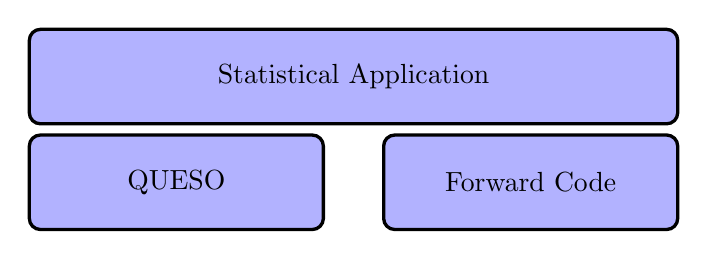
\begin{tikzpicture}[
      desc/.style={
        rectangle,
        rounded corners,
        draw=black,
        very thick,
        text centered,
        text width=8cm,
        minimum height=12mm,
        fill=blue!30
      }
    ]

    \node [desc] (StatApp) {Statistical Application};
    \node [desc, text width=3.5cm, anchor=north west, yshift=-1mm] (QUESO) at (StatApp.south west) {QUESO};
    \node [desc, text width=3.5cm, anchor=north east, yshift=-1mm] (Fwd) at (StatApp.south east) {Forward Code};

    \end{tikzpicture}
  \end{figure}
\end{frame}

\begin{frame}{Preliminaries}
  \begin{itemize}
    \item Instructions on how to build and install \Queso: \url{http://libqueso.com}
    \item All \Queso\ docs are here: \url{http://libqueso.com/queso/html/}.
    \item Links on these slides are clickable
    \item I'm British, so I spell things weird.  \Queso\ uses American English.
      \begin{itemize}
        \item It's a hard habit for me to break, so be cognizant of potential
          spelling differences in the code on these slides
        \item Try to compile stuff as we go along
      \end{itemize}
    \item These slides will not take four hours to deliver:
      \begin{itemize}
        \item There are hands-on tasks you can do.  Please do them.
        \item I encourage interruptions for questions or comments.
      \end{itemize}
    \item There are some areas of \Queso\ I am not familiar with.  I will only
      talk about the areas I am familiar with.
  \end{itemize}
\end{frame}

\section{The environment}
\begin{frame}[fragile]{The environment}
  \begin{itemize}
    \item All classes are available in the \texttt{QUESO} namespace.
    \item Most of the objects in \Queso\ need an \emph{environment}.
    \item Some objects can infer it from other objects.
    \item Lives in \texttt{queso/Enivornment.h} and called \texttt{FullEnvironment}.
  \end{itemize}
  \begin{verbatim}
#include <queso/Environment.h>

int main(int argc, char ** argv)
{
  QUESO::FullEnvironment env(MPI_COMM_WORLD, argv[1], "",
                             NULL);
  return 0;
}
  \end{verbatim}
\end{frame}

\begin{frame}[fragile]{The environment}
  \begin{verbatim}
QUESO::FullEnvironment env(MPI_COMM_WORLD, argv[1], "",
                           NULL);
  \end{verbatim}
  Arguments:
  \begin{enumerate}
    \item \Mpi\ communitcator.
    \item Path to \Queso\ input file.
    \item Prefix string for entries in the input file.
    \item Optional programatically provided input options.
  \end{enumerate}
\end{frame}

\section{Task 1}
\begin{frame}[fragile]{Task 1}
  \begin{itemize}
    \item Create a source file and instantiate a \texttt{FullEnvironment}.
    \item Compile it, link it against \Queso\ and run it.
    \item  Make sure there are no errors.
    \item You might need an input file.  You can find one here:
      \url{https://github.com/libqueso/queso/blob/dev/examples/template_example/template_example_input.txt}
    \item We'll talk about the input file later.  For now you can take it for
      granted.
    \item This task should take less than five minutes.
  \end{itemize}
\end{frame}

\section{Vectors}
\begin{frame}[fragile]{Vectors}
  \begin{itemize}
    \item Vectors live in a vector space.
    \item Most classes in \Queso\ are templated around vector implementation.
    \item The default vector/matrix implementation is \Gsl.
  \end{itemize}
  \begin{verbatim}
QUESO::VectorSpace<> paramSpace(env, "param_", 1, NULL);
  \end{verbatim}
  Arguments:
  \begin{itemize}
    \item The environment.
    \item The prefix for input file items.
    \item The dimension of the vector space.
    \item A pointer to a \texttt{std:vector} of \texttt{std:string}s for naming
      components of the vectors.  Good for `naming' parameters.
  \end{itemize}
\end{frame}

\begin{frame}[fragile]{Vectors}
  In \Queso\ \texttt{v0.53.x}, the following classes are equivalent:
  \begin{verbatim}
QUESO::VectorSpace<>
QUESO::VectorSpace<QUESO::GslVector, QUESO::GslMatrix>
  \end{verbatim}
  \begin{itemize}
    \item The default template type is
      \texttt{QUESO::GslVector}/\texttt{QUESO::GslMatrix}.
    \item The \Queso\ development team are working closely with the
      \texttt{DAKOTA} team at Sandia to provide a wider range of
      high-perfomance vector/matrix implementations in the 12--15 month
      timeline.
    \item If you really don't like \texttt{QUESO::} everywhere, you can
      insert
      \begin{verbatim}
using namespace QUESO;
      \end{verbatim}
       in your code and remove all instances of \texttt{QUESO::} elsewhere.
  \end{itemize}
\end{frame}

\begin{frame}[fragile]{Vectors}
  This \texttt{zeroVector} method returns a \texttt{GslVector} object belonging
  to the vector space with every component set to zero.
  \begin{verbatim}
paramSpace.zeroVector();
  \end{verbatim}
  Use the vector space to eke out the zero vector, then copy it.
  \begin{verbatim}
QUESO::GslVector myVector(paramSpace.zeroVector());
  \end{verbatim}
  Argument is another \texttt{GslVector} object.
\end{frame}

\begin{frame}[fragile]{Vectors}
  Set element \texttt{3}:
  \begin{verbatim}
myVector[2] = 1.0;
  \end{verbatim}
  Get element \texttt{2}:
  \begin{verbatim}
double myElement = myVector[1];
  \end{verbatim}
  Set every element to \texttt{5.0}:
  \begin{verbatim}
myVector.cwSet(5.0);
  \end{verbatim}
  For other methods, see \url{http://libqueso.com/queso/html/a00129.html}
\end{frame}

\section{Matrices}
\begin{frame}[fragile]{Matrices}
  \begin{itemize}
    \item All matrices are square.
    \item Obviously not true, but most of the time we only care about square
      (covariance) matrices.
    \item You can create nonsquare matrices, but I doubt you will ever need
      one in \Queso\ unless your forward problem needs it.
    \item Matrices don't \emph{live} in the vector space, but they are defined
      over it.
    \item Use an existing \texttt{GslVector} to construct a square matrix with
      compatible dimension.
  \end{itemize}
  \begin{verbatim}
QUESO:GslMatrix myMatrix(myVector);
  \end{verbatim}
  \begin{itemize}
    \item Creates diagonal matrix with element $(i, i)$ equal to
      \texttt{myVector[i]}.
    \item Argument is a \texttt{GslVector} object but could be another
      \texttt{GslMatrix}, in which case the whole matrix is copied.
  \end{itemize}
\end{frame}

\begin{frame}[fragile]{Matrices}
  Set element $(3, 4)$:
  \begin{verbatim}
myMatrix(2, 3) = 1.0;
  \end{verbatim}
  Get element $(2, 3)$:
  \begin{verbatim}
double myElement = myMatrix(1, 2);
  \end{verbatim}
  \begin{itemize}
    \item \Queso\ has methods that can factorise matrices in order to solve
      linear systems.
    \item Linear algebra all relies on \Gsl.
    \item See above comment about ongoing work for high-performance
      vector/matrix implementations.
    \item For other methods, see
      \url{http://libqueso.com/queso/html/a00127.html}
  \end{itemize}
\end{frame}

\section{Task 2}
\begin{frame}[fragile]{Task 2}
  \begin{itemize}
    \item Create a \texttt{GslVector}.
    \item Create a \texttt{GslMatrix}.
    \item Multiply the vector by the matrix.
    \item Verify the result of the multiplication is correct.
    \item If you complete this quickly, look at the documentation and play with
      some of the other methods.
    \item This task should take less than ten minutes.
  \end{itemize}
\end{frame}

\section{Parameter domains}
\begin{frame}[fragile]{Parameter domains}
  \begin{itemize}
    \item Random variables are defined on a `state space' or `domain'.
    \item State space may be a proper subset of the whole vector space
      \texttt{paramSpace}.
    \item Most domains are boxes.
    \item More exotic domains are not supported out of the box.
    \item Creating your own will not be covered here.
  \end{itemize}
  \begin{verbatim}
QUESO::GslVector paramMins(paramSpace.zeroVector());
QUESO::GslVector paramMaxs(paramSpace.zeroVector());
paramMins.cwSet(0.0);
paramMaxs.cwSet(1.0);

QUESO::BoxSubset<> paramDomain("param_", paramSpace,
                               paramMins, paramMaxs);
  \end{verbatim}
\end{frame}

\begin{frame}[fragile]{Parameter domains}
  \begin{verbatim}
QUESO::BoxSubset<> paramDomain("param_", paramSpace,
                               paramMins, paramMaxs);
  \end{verbatim}
  Arguments are:
  \begin{enumerate}
    \item Prefix for input file entries.
    \item The underlying vector space that elements of the domain belong to.
    \item A vector of the minimum values in each dimension.
    \item A vector of the maximum values in each dimension.
  \end{enumerate}
  \textbf{Note:} Passing \texttt{INFINITY} (\texttt{-INFINITY}) as the maximum
  (minimum) of the domain limits is allowed.
\end{frame}

\section{Random variables}
\begin{frame}[fragile]{Random variables}
  \begin{itemize}
    \item \Queso\ supports the following random variables:
      \begin{itemize}
        \item Inverse Gamma
        \item Jeffreys
        \item Log Normal
        \item Beta
        \item Gamma
        \item Gaussian
        \item Uniform
        \item Wigner
      \end{itemize}
    \item \Queso also supports creating custom random variables.
  \end{itemize}
\end{frame}

\begin{frame}[fragile]{Random variables}
  \begin{itemize}
    \item Random variables need the domain, and possibly other parameters
    \item Uniform:
      \begin{verbatim}
QUESO::UniformVectorRV<> priorRv("prior_", paramDomain); \end{verbatim}
    \item Beta needs a vector of $\alpha$ and $\beta$ parameters as well:
      \begin{verbatim}
QUESO::BetaVectorRV<> betaRv("prior_", paramDomain,
                             alphas, betas);\end{verbatim}
    \item Gaussians need a mean and covariance:
      \begin{verbatim}
QUESO::GaussianVectorRV<> gaussianRv("prior_",
                                     paramDomain, mean,
                                     cov); \end{verbatim}
    \item Unless it's obvious how to correlated elements of the vector, they
      are assumed to be independent.
  \end{itemize}
\end{frame}

\begin{frame}[fragile]{Random variables}
  \begin{itemize}
    \item \texttt{*VectorRV} classes have two major components:
      \begin{itemize}
        \item A \texttt{*JointPdf} object to evaluate the underlying density.
        \item A \texttt{*VectorRealizer} component to draw realisations.
      \end{itemize}
    \item You can access these components with the \texttt{pdf()} method\ldots
      \begin{verbatim}
QUESO::GslVector point(paramSpace.zeroVector());
betaRv.pdf().actualValue(point, NULL, NULL, NULL,
                         NULL); \end{verbatim}
    \item \ldots or the \texttt{realizer()} method
      \begin{verbatim}
QUESO::GslVector draw(paramSpace.zeroVector());
betaRv.realizer().realization(draw); \end{verbatim}
  \end{itemize}
\end{frame}

\section{Task 3}
\begin{frame}[fragile]{Task 3}
  \begin{enumerate}
    \item Create a Guassian random variable over some domain.
    \item Think about your domain for a few minutes.
    \item Compute (and print) the empirical mean and variance (see point 2.)
      from $10^6$ realisations.
    \item Are they (approximately) what you expect them to be?  If not, why
      not?
    \item This task should take less than fifteen minutes.
  \end{enumerate}
\end{frame}

\section{Likelihoods}
\begin{frame}[fragile]{Likelihoods}
  \begin{itemize}
    \item We now know enough to define our own prior random variable.
    \item For standard MCMC, we don't need \emph{realisations} from the
      prior.  Only need \emph{pdf evaluations}.
    \item Since all random variables in \Queso\ have a \texttt{pdf()} method,
      that's what \Queso\ will use to evaluate the prior pdf when sampling.
    \item Up next is the likelihood.
    \item There are no out-of-the-box likelihoods in \Queso, because they need
      the \emph{forward problem}!
    \item We will write an example forward problem first, and then create a
      likelihood function in \Queso\ to evaluate the forward problem.
    \item Then we'll give the prior and likelihood to \Queso.
    \item \Queso\ will then solve the Bayesian problem.
  \end{itemize}
\end{frame}

\begin{frame}{General framework}
  Model (usually a PDE): $\mathcal{G}(\theta)$ where $\theta$ are model
  paramaters.
  \linebreak
  \linebreak
  Observations:
  \begin{equation*}
    y = \mathcal{G}(\theta) + \eta, \quad \eta \sim \mathcal{N}(0, R)
  \end{equation*}
  Want:
  \begin{align*}
    p(\theta | y) &\propto p(y | \theta) p(\theta) \\
    &\propto \exp \left( -\frac12 \| \mathcal{G}(\theta) - y \|^2_R \right)
    \exp \left( -\frac12 \| \theta - \bar{\theta} \|^2 \right)
  \end{align*}
  \textbf{Note:} The last proportionality is only true for Gaussian noise and
  Gaussian prior.
\end{frame}

\begin{frame}{What does MCMC look like?}
  \begin{figure}[htp]
    \tikzstyle{vertex}=[circle,minimum size=3pt,inner sep=0pt]
    \begin{tikzpicture}[scale=1.0,y=\textwidth/2.0, x=\textwidth/8.0]
      % axis
      \draw (-4,0) -- coordinate (x axis mid) (4,0);
      % plot
      \draw[color=blue] plot[smooth] file{pdf.dat};
      \foreach \pos / \name / \fra in {{(2,0)/a/1}, {(1.75,0)/b/1}, {(1.5,0)/c/2}, {(1.25, 0)/d/3},
                        {(1,0)/e/4}, {(0.75,0)/f/5}, {(0.5,0)/g/6}, {(0.2,0)/h/7},
                        {(0.4198968,0)/i/8}, {(1.89466061,0)/j/9}, {(-1.19766853,0)/k/10},
                        {(-1.32317683,0)/l/11}, {(1.68164494,0)/m/12}, {(1.0415304,0)/n/13},
                        {(-0.71843111,0)/o/14}, {(1.71829706,0)/p/15}, {(-0.31911559,0)/q/16},
                        {(-0.4858966,0)/r/17}}
      \node<\fra->[vertex,fill=red] (\name) at \pos{};
      \foreach \source / \dest / \fr in {a/b/1, b/c/2, c/d/3, d/e/4, e/f/5, f/g/6, g/h/7, h/i/8, i/j/9, j/k/10, k/l/11,
                                   l/m/12, m/n/13, n/o/14, o/p/15, p/q/16, q/r/17}
      \draw<\fr>[red,->] (\source) .. controls +(0,-0.1) and +(0,-0.1) .. (\dest);
      \phantom{\draw<18>[red,->] (a) .. controls +(0,-0.1) and +(0,-0.1) .. (b);}
      \node<18-> (mean) at (-2.3, 0.75) {$\mathbb{E}(\theta | y ) \approx \frac{1}{N} \sum_{k=1}^{N} \theta_k$};
      \path (0, 0) coordinate (origin);
      \draw<18->[black,->, thick] (mean) .. controls (-2.5,0.2) and (0,0.2) .. (origin);
    \end{tikzpicture}
  \end{figure}
\end{frame}

\begin{frame}{How to do MCMC?  Sampling $p(\theta | y)$}
  \begin{itemize}
  \item Idea: Construct $\{ \theta_k \}_{k = 1}^{\infty}$ cleverly such that
    $\{ \theta_k \}_{k = 1}^{\infty} \sim p(\theta | y)$
    \begin{enumerate}
    \item Let $\theta_j$ be the `current' state in the sequence and construct a \textit{proposal}, $z \sim q(\theta_j, \cdot)$
    \item<2-> \uncover<2->{Compute $\alpha(\theta_j, z) = 1 \wedge \frac{p(z |  y) q(z, \theta_j)}{p(\theta_j | y) q(\theta_j, z)}$}
    \item<3-> \uncover<3->{
        Let
        \begin{gather*}
          \theta_{j+1} =
            \begin{cases}
              \theta   & \mbox{with probability } \alpha(\theta_j, z) \\
              \theta_j & \mbox{with probability } 1 - \alpha(\theta_j, z)
            \end{cases}
        \end{gather*}
      }
    \end{enumerate}
  \item<4-> \uncover<4->{We can take $\theta_1$ to be a draw from $p(\theta)$}
  \end{itemize}
\end{frame}

\begin{frame}[fragile]{Likelihoods}
  \begin{itemize}
    \item To create a custom likelihood, we will subclass \texttt{BaseScalarFunction}.
    \item We will implement \texttt{lnValue} and \texttt{actualValue}.
    \item Sublass like so:
      \begin{verbatim}
template<class V, class M>
class Likelihood : public QUESO::BaseScalarFunction<V, M>
{ \end{verbatim}
    \item You can call your class whatever you want, but \texttt{Likelihood}
      seemed like a good name.
  \end{itemize}
\end{frame}

\begin{frame}[fragile]{Likelihoods}
  \begin{itemize}
    \item Implement the \emph{constructor}:
      \begin{verbatim}
Likelihood(const char * prefix,
           const QUESO::VectorSet<V, M> & domain)
  : QUESO::BaseScalarFunction<V, M>(prefix, domain)
{
// Setup here
} \end{verbatim}
    \item The constructor is called when you create an object of type
      \texttt{Likelihood}.
  \end{itemize}
\end{frame}

\begin{frame}[fragile]{Likelihoods}
  \begin{itemize}
    \item Implement the \emph{destructor}:
      \begin{verbatim}
virtual ~Likelihood(
{
  // Deconstruct here
} \end{verbatim}
    \item The destructor is called when your creates object of type
      \texttt{Likelihood} goes out of scope.
    \item Do all cleanup in the destructor.
  \end{itemize}
\end{frame}

\begin{frame}[fragile]{Likelihoods}
  \begin{itemize}
    \item Implement the \texttt{lnValue} method:
      \begin{verbatim}
virtual double lnValue(const V & domainVector,
  const V * domainDirection, V * gradVector,
  M * hessianMatrix, V * hessianEffect) const
{
  double diff = G(domainVector[0]) - m_observations[0];
  return -0.5 * diff * diff / (sigma * sigma);
} \end{verbatim}
    \item \texttt{lnValue} should return $\log$ of $p(\theta | y)$ at the point
      $\theta =$ \texttt{domainVector}.
    \item You also need to implement \texttt{actualValue} but you can just
      return \texttt{std::exp(lnValue(...))}.
  \end{itemize}
\end{frame}

\section{Task 4}
\begin{frame}[fragile]{Task 4}
  \begin{itemize}
    \item We'll use an example forward model in Chemistry called the Massman
      model:
      \begin{equation*}
        \mathcal{G}(D, \beta) = D T^{\beta}
      \end{equation*}
    \item Uncertain parameters are $\theta = (D, \beta)$.  Observations are
      taken at $T = 313.7, 314.9, 375.2, 474.7, 481.0, 573.5, 671.1$
    \item Observation vector is $y = (4603.50, 4638.15, 6302.27, 9505.89,
      9755.11, 13239.08, 17431.02)$
    \item Observational error is Gaussian and standard deviation is $10.0$.
    \item Create your own likelihood for this forward problem.
    \item Instantiate it.
    \item Make sure you can evaluate it at a point in parameter space.
    \item This task should talk less than thirty minutes.
  \end{itemize}
\end{frame}

\section{Statistical inverse problem}
\begin{frame}[fragile]{Statistical inverse problem}
  \begin{itemize}
    \item So far, have created a prior
    \item Have created a likelihood
    \item We will now from the statistical inverse problem
    \item \Queso\ will solve the statistical inverse problem
  \end{itemize}
\end{frame}

\begin{frame}[fragile]{Statistical inverse problem}
  Create a posterior random variable (on the same domain):
  \begin{verbatim}
QUESO::GenericVectorRV<> postRv("post_", paramSpace); \end{verbatim}
  Create a statistical inverse problem with the prior, likelihood and
  posterior:
  \begin{verbatim}
QUESO::StatisticalInverseProblem<> ip("", NULL,
                                      priorRv,
                                      lhood, postRv); \end{verbatim}
\end{frame}

\begin{frame}[fragile]{Statistical inverse problem}
  Before we solve the problem we have to tell \Queso\ what the first sample in
  the chain is:
  \begin{verbatim}
QUESO::GslVector paramInitials(paramSpace.zeroVector());
paramInitials[0] = 1.0;
paramInitials[1] = 1.0; \end{verbatim}
  And we also have to tell \Queso\ the variance of the proposal distribution:
  \begin{verbatim}
QUESO::GslMatrix propCovMatrix(paramSpace.zeroVector());
propCovMatrix(0, 0) = 0.0001;
propCovMatrix(1, 1) = 0.0001; \end{verbatim}
  These are algorithmic knobs, and there are efforts to remove this necessity
  in future and start with sensible defaults.  For now, though, we have to set
  these.
\end{frame}

\begin{frame}[fragile]{Statistical inverse problem}
  Now solve and tidy up:
  \begin{verbatim}
  ip.solveWithBayesMetropolisHastings(NULL, paramInitials,
                                      &propCovMatrix);
  MPI_Finalize();
  return 0;
} \end{verbatim}
\end{frame}

\section{Task 5}
\begin{frame}[fragile]{Task 5}
  \begin{itemize}
    \item Compile and run the code.  Output will be in the \texttt{outputData} directory
    \item Samples are stored in the \texttt{ip\_raw\_chain\_.m} file as a
      \texttt{matlab} vector
    \item The first column are samples of the first parameter
      (\texttt{domainVector[0]}).  The second column are samples of the second
      parameter (\texttt{domainVector[1]})
    \item Matlab output is a hinderance (not open source).  There are efforts
      to output an HDF5 file in future.  Initial support exists but is not
      usable at present
    \item Use script to plot the samples to a PDF file.
    \item The truth is $(D, \beta) = (0.197, 1.75)$.
    \item Plot the running mean and variance of the samples.  What do you get?
    \item This task should take less than twenty minutes.
  \end{itemize}
\end{frame}

\section{Analysing output}
\begin{frame}[fragile]{\Queso\ output}
  \begin{itemize}
    \item At this point, you should be able to see your samples.
    \item Are they correct?
    \item Should look like white noise
    \item Steps or large meanderings is considered transient behaviour
    \item An initial transient period is ok (see later) but it should settle
      down
    \item If there is an initial transient period, do not include this period
      when calculating mean, variance, other moments
    \item There are more quantitative convergence metrics: autocorrelation,
      Geweke, effective sample size, Raftery and Lewis, Heidelberger and Welch,
      Gelman and Rubin.
    \item See here for details: \url{https://support.sas.com/documentation/cdl/en/statug/63033/HTML/default/viewer.htm#statug_introbayes_sect008.htm}
  \end{itemize}
\end{frame}

\begin{frame}[fragile]{\Queso\ output: Autocorrelation}
  Autocorrelation of chain:
  \begin{figure}
    \begin{center}
      \includegraphics[width=0.85\textwidth]{autocorrs.pdf}
    \end{center}
  \end{figure}
\end{frame}

\begin{frame}[fragile]{\Queso\ output: Autocorrelation}
  Autocorrelation of white noise:
  \begin{figure}
    \begin{center}
      \includegraphics[width=0.85\textwidth]{autocorrs_white_noise.pdf}
    \end{center}
  \end{figure}
  Time taken for autocorrelation to decay is a measure of Markov chain mixing
  efficiency.  `Mixing' is how well the Markov chain explores the state space.
\end{frame}

\begin{frame}[fragile]{\Queso\ output: Geweke diagnostic}
  Take averages of chunk of samples from beginning and end separately:
  \begin{align*}
    \bar{D}_1 &= \frac{1}{n_1} \sum_{i=1}^{n_1} D_i \\
    \bar{D}_2 &= \frac{1}{n_2} \sum_{i=n - n_2 + 1}^{n} D_i
  \end{align*}
  The distribution of the random variable $\bar{D}_1 - \bar{D}_2$ converges to
  a normal distribution with mean zero.
\end{frame}

\begin{frame}[fragile]{\Queso\ output: Geweke diagnostic}
  \begin{figure}
    \begin{center}
      \includegraphics[width=0.85\textwidth]{geweke.pdf}
    \end{center}
  \end{figure}
\end{frame}

\begin{frame}[fragile]{Other \Queso\ output}
  \begin{itemize}
    \item Other useful output is produced by \Queso.
    \item Should be reasonably obviously named, but:
      \begin{itemize}
        \item log-likelihood values at each sample in the chain:
          \texttt{ip\_raw\_chain\_loglikelihood.m}
        \item log-target values at each sample in the chain:
          \texttt{ip\_raw\_chain\_logtarget.m}
        \item General diagnostic information and logging information that
          \Queso\ encounters:
          \texttt{display\_sub0.txt}
        \item Algorthmic information about the inverse problem:
          \texttt{sipOutput.m}
          \begin{itemize}
            \item Proportion of rejected samples is written here
          \end{itemize}
      \end{itemize}
  \end{itemize}
\end{frame}

\section{Running \Queso\ in parallel}
\begin{frame}[fragile]{Parallel \Queso}
  \begin{itemize}
    \item Have been running with \texttt{./binary inputfile.txt}
    \item This is equivalent to \texttt{mpirun -np 1 ./binary inputfile.txt}
    \item Want to do \texttt{mpirun -np N ./binary inputfile.txt}
    \item \texttt{N = 2} will tell \Queso\ to give the sampler two processes
    \item But still only one chain produced!  Why?
    \item The usecase for this would be if the \emph{forward problem} needed
      two processes per evaluation
  \end{itemize}
\end{frame}

\begin{frame}{Parallel \Queso}
  \begin{figure}
    \centering
    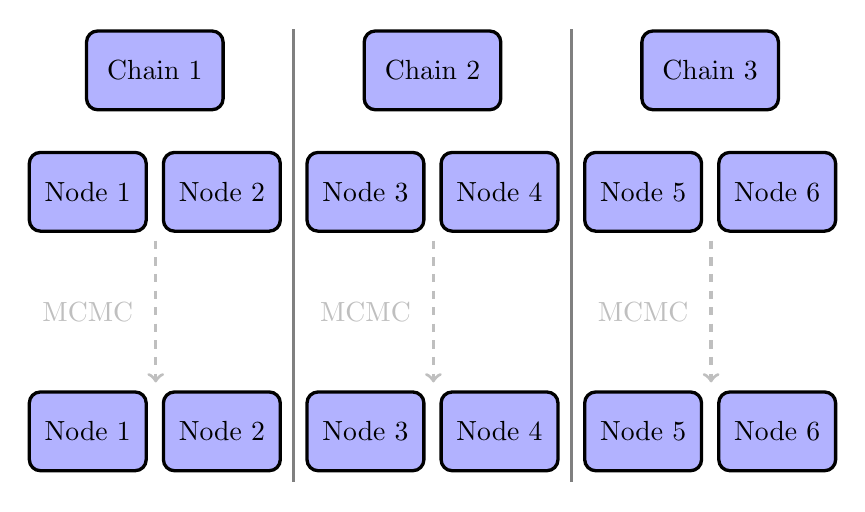
\begin{tikzpicture}[
      desc/.style={
        rectangle,
        rounded corners,
        draw=black,
        very thick,
        text centered,
        text width=8cm,
        minimum height=10mm,
        fill=blue!30
      }
    ]

    % Chains
    \node[desc, text width=1.5cm, anchor=east, xshift=1.75cm] (Chain1) {Chain 1};
    \node[desc, text width=1.5cm, anchor=west, xshift=1.75cm] (Chain2) at (Chain1.east) {Chain 2};
    \node[desc, text width=1.5cm, anchor=west, xshift=1.75cm] (Chain3) at (Chain2.east) {Chain 3};

    % Separators
    % \draw [very thick,-,gray] (Chain1.south west) ++(0,-0.4) -- ++(0,-5);
    \draw[very thick,-,gray] (Chain1.north east) ++(0.875,0) -- ++(0,-5.75);
    \draw[very thick,-,gray] (Chain2.north east) ++(0.875,0) -- ++(0,-5.75);

    % Nodes in chain 1
    \node[desc, text width=1.25cm, anchor=north east, xshift=8mm, yshift=-5mm] (Node1) at (Chain1.south west) {Node 1};
    \node[desc, text width=1.25cm, anchor=north west, xshift=-8mm, yshift=-5mm] (Node2) at (Chain1.south east) {Node 2};

    % Nodes in chain 2
    \node[desc, text width=1.25cm, anchor=north east, xshift=8mm, yshift=-5mm] (Node3) at (Chain2.south west) {Node 3};
    \node[desc, text width=1.25cm, anchor=north west, xshift=-8mm, yshift=-5mm] (Node4) at (Chain2.south east) {Node 4};

    % Nodes in chain 3
    \node[desc, text width=1.25cm, anchor=north east, xshift=8mm, yshift=-5mm] (Node5) at (Chain3.south west) {Node 5};
    \node[desc, text width=1.25cm, anchor=north west, xshift=-8mm, yshift=-5mm] (Node6) at (Chain3.south east) {Node 6};

    % Nodes in chain 1 after mcmc iter
    \node[desc, text width=1.25cm, anchor=north, yshift=-2cm] (Node11) at (Node1.south) {Node 1};
    \node[desc, text width=1.25cm, anchor=north, yshift=-2cm] (Node21) at (Node2.south) {Node 2};

    % Nodes in chain 2 after mcmc iter
    \node[desc, text width=1.25cm, anchor=north, yshift=-2cm] (Node31) at (Node3.south) {Node 3};
    \node[desc, text width=1.25cm, anchor=north, yshift=-2cm] (Node41) at (Node4.south) {Node 4};

    % Nodes in chain 3 after mcmc iter
    \node[desc, text width=1.25cm, anchor=north, yshift=-2cm] (Node51) at (Node5.south) {Node 5};
    \node[desc, text width=1.25cm, anchor=north, yshift=-2cm] (Node61) at (Node6.south) {Node 6};

    % MCMC arrows
    \draw[very thick,->,dashed,lightgray] (Node1.south east) ++(0.1,-0.1) -- ++(0,-1.8);
    \draw[very thick,->,dashed,lightgray] (Node3.south east) ++(0.1,-0.1) -- ++(0,-1.8);
    \draw[very thick,->,dashed,lightgray] (Node5.south east) ++(0.1,-0.1) -- ++(0,-1.8);

    % MCMC text
    \node[yshift=-1cm,text=lightgray] at (Node1.south) {MCMC};
    \node[yshift=-1cm,text=lightgray] at (Node3.south) {MCMC};
    \node[yshift=-1cm,text=lightgray] at (Node5.south) {MCMC};
    \end{tikzpicture}
  \end{figure}
\end{frame}

\begin{frame}[fragile]{Parallel \Queso}
  \begin{itemize}
    \item The number of chains can be increased from the input file.  Change:
      \begin{verbatim}
    env_numSubEnvironments = 1 \end{verbatim}
      to
      \begin{verbatim}
    env_numSubEnvironments = 4 \end{verbatim}
      for four chains.
    \item For one process per chain, run with \texttt{mpirun -np 4}
    \item For two prorcesses per chain, run with \texttt{mpirun -np 2}
    \item \Queso\ will check if \texttt{env\_numSubEnvironments} divides
      the size of \texttt{MPI\_COMM\_WORLD}
    \item If not, an exception is thrown
  \end{itemize}
\end{frame}

\begin{frame}[fragile]{Parallel \Queso}
  \begin{itemize}
    \item When multiple \texttt{subEnvironments} are asked for, multiple output
      files are produced
    \item The output files for \texttt{subEnvironment} $N+1$ are prefixed with
      \texttt{\_subN} before the file extension
    \item Example: raw chain samples from process 3 are in
      \texttt{ip\_raw\_chain\_sub2.m}
    \item Example: log-likelihood values at each raw chain sample from process
      2 are in \texttt{ip\_raw\_chain\_loglikelihood\_sub1.m}
    \item \Queso\ automatically concatenates, in order of increasing
      \texttt{subEnvironment} index, each raw chain and saves it to
      \texttt{ip\_raw\_chain.m} so this file will contain the number of samples
      per \texttt{subEnvironment} multiplied by the number of
      \texttt{subEnvironments}.
  \end{itemize}
\end{frame}

\section{The \Queso\ input file}
\begin{frame}[fragile]{\Queso\ input file: Environment options}
  \begin{itemize}
    \item Already seen how to change number of chains with input file
    \item Prefix stuff is here.  \texttt{env\_} is the default prefix is empty
      for the \texttt{FullEnvironment}.  You can change it and the
      input file options will need to be prefixed with the passed user prefix.
    \item Some environment options:
      \begin{itemize}
        \item \texttt{env\_subDisplayFileName} is the place to \Queso\ will
          put general diagnostic information
        \item \texttt{env\_subDisplayAllowAll} toggles whether or not all
          process can write output related to environment
        \item \texttt{env\_subDisplayAllowedSet} if the above option is false,
          this option allows you to specify a subset of processes that can
          write output
        \item \texttt{env\_seed} is a flag for setting random number generator
          seed.  Set this to something negative if you want multiple concurrent
          chains to produce distinct samples.  If nonzero, this is the seed
          that is used for all chains.
      \end{itemize}
  \end{itemize}
\end{frame}

\begin{frame}[fragile]{\Queso\ input file: Inverse problem options}
  \begin{itemize}
    \item Inverse problem options
      \begin{itemize}
        \item \texttt{ip\_computeSolution} is a boolean.  If false, no
          computation of the inverse problem is done.  Useful for testing
          setup.
        \item \texttt{ip\_dataOutputFileName} is the output file for inverse
          problem related information.
        \item \texttt{ip\_dataOutputAllowedSet} similar to environment option,
          but specific to inverse problem
      \end{itemize}
  \end{itemize}
\end{frame}

\begin{frame}[fragile]{\Queso\ input file: Algorithm options}
  \begin{itemize}
    \item All DRAM options are documented as part of the
      \texttt{MhOptionsValues} class
      \begin{itemize}
        \item \url{http://libqueso.com/queso/html/a00166.html}
      \end{itemize}
    \item Software documentation and usability is assessed by users
    \item If there are any options (anywhere, not just DRAM) that are unclear
      or undocumented feel free to open a new GitHub ticket
    \item Better yet, write a patch to fix it and you can be a \Queso\
      contributor!
  \end{itemize}
\end{frame}

\begin{frame}[fragile]{Programmatically setting options}
  \begin{itemize}
    \item You can set options programmatically instead of via the input file
    \item Objects whose behaviour is tweakable will accept a pointer to an
      instance of \texttt{*OptionsValues} in the constructor
      \begin{itemize}
        \item \texttt{FullEnvironment} takes an \texttt{EnvOptionsValues}
          pointer: \url{http://libqueso.com/queso/html/a00081.html#a77081a9fd8cb7b90ee3c0da289d91815}
        \item \texttt{StatisticalInverseProblem} takes an
          \texttt{SipOptionsValues} pointer: \url{http://libqueso.com/queso/html/a00207.html#a98ad98a7030b2c6577a0e840506bf74d}
        \item Options object member names are similar to input file option names
      \end{itemize}
    \item You needn't create a \texttt{MetropolisHastingsSG} object; the
      inverse problem will create one for you
    \item You can pass options via \texttt{solveWithBayesMetropolisHastings}:
      \begin{itemize}
        \item \url{http://libqueso.com/queso/html/a00207.html#a924189e647110129682308b9bffc3a0d}
      \end{itemize}
  \end{itemize}
\end{frame}

\begin{frame}[fragile]{Thinning}
  \begin{itemize}
    \item A common way to try and improve decorrelation time is by thinning
    \item Thinning is simply saving every $m$-th sample where $m > 1$
    \item The \texttt{ip\_raw\_chain.m} contains the unthinned chain
    \item To enable thinning, turn on this input file option:
      \begin{itemize}
        \item \texttt{ip\_mh\_filteredChain\_generate = 1}
      \end{itemize}
    \item With this option on, you must also set the value for $m$:
      \begin{itemize}
        \item \texttt{ip\_mh\_filteredChain\_lag = 2}
      \end{itemize}
    \item Somewhere to store the output:
      \begin{itemize}
        \item \texttt{ip\_mh\_filteredChain\_dataOutputFileName = outputData/ip\_filtered\_chain}
      \end{itemize}
    \item Let all processes write their output
      \begin{itemize}
        \item \texttt{ip\_mh\_filteredChain\_dataOutputAllowAll = 1}
      \end{itemize}
  \end{itemize}
\end{frame}

\section{Task 6}
\begin{frame}[fragile]{Task 6}
  \begin{itemize}
    \item Enable thinning
    \item Perhaps remove (or backup) the existing \texttt{outputData} directory
    \item Run the code (perhaps with multiple chains in parallel)
    \item Verify the length of the filtered chain is what you expect
    \item Compute the running mean of the samples.  Does it converge faster
      or slower?
    \item This task should take less than twenty minutes.
  \end{itemize}
\end{frame}

\section{Extras}
\begin{frame}[fragile]{Some useful DRAM options}
  \begin{itemize}
    \item \texttt{ip\_mh\_putOutOfBoundsInChain}:  If true, can be wasteful in
      high-dimensional bounded domains.
    \item \texttt{ip\_mh\_doLogitTransform}:  Transforms bounded domain to
      unbounded domain for efficiency in high dimensions.
    \item \texttt{ip\_mh\_dr\_maxNumExtraStages}:  Number of DR stages to do.
      Can improve mixing.  More stages requires more likelihood evaluations.
    \item \texttt{ip\_mh\_dr\_listOfScalesForExtraStages}:  A list of inverse
      scale factors to scale the proposal covariance matrix by in each DR
      stage.
    \item \texttt{ip\_mh\_am\_initialNonAdaptInterval}:  Number of iterations
      to not adapt.
    \item \texttt{ip\_mh\_am\_adaptInterval}:  The frequency at which to adapt
      proposal covariance matrix (after initial non-adapt period is over).
  \end{itemize}
\end{frame}

\begin{frame}[fragile]{Optimisation}
  \begin{itemize}
    \item \Queso\ can optimise, using deterministic optimisation tools in \Gsl,
      to find the MAP estimator before sampling
    \item Better than starting from a user-defined initial sample, or from a
      realisation from the prior
    \item Caveat:  not all problems are easily optimised
    \item If no derivative provided, then finite differences are used
    \item The default tweakable optimisation parameters are hardcoded.  There is
      an open ticket to change this, but it needs work:
      \url{https://github.com/libqueso/queso/pull/310}
    \item To enable optimisation, call \texttt{seedWithMAPEstimator()} before
      calling \texttt{solveWithBayesMetropolisHastings(\ldots)}.
  \end{itemize}
\end{frame}

\section{Contributing}
\begin{frame}[fragile]{Contributing}
  \begin{itemize}
    \item All software has bugs
    \item \Queso\ is open source software, so it is free
    \item Free means you don't have to pay for it (beer)
    \item Free also means you are free to play with the source code yourself
      (speech)
    \item If you use \Queso\ and you need help, please email the users mailing
      list
      \begin{itemize}
        \item \url{queso-users@googlegroups.com}
      \end{itemize}
    \item To stay apprised of new releases or discuss future directions email
      the developers list
      \begin{itemize}
        \item \url{queso-dev@googlegroups.com}
      \end{itemize}
    \item You can also help others that ask questions on these lists
    \item Community contribution
  \end{itemize}
\end{frame}

\begin{frame}[fragile]{Contributing}
  \begin{itemize}
    \item If you use \Queso\ and you encounter a bug, open a ticket
      \begin{itemize}
        \item \url{https://github.com/libqueso/queso/issues/new}
      \end{itemize}
    \item If you fix a bug and want to contribute to the \Queso\ codebase
      \begin{itemize}
        \item Awesome
        \item Review contribution guidelines here:
          \url{https://github.com/libqueso/queso#contributing}
        \item Write tests for your patches
        \item And if you add a new feature, make sure to write documentation
      \end{itemize}
  \end{itemize}
\end{frame}

\section{Future work}
\begin{frame}[fragile]{The future of \Queso}
  \begin{itemize}
    \item \Queso\ works closely with the DAKOTA team at Sandia
      \begin{itemize}
        \item They provide feedback on our design
        \item They request features
        \item They find bugs
        \item We learn from their (software and optimisation) expertise
        \item DAKOTA can link to \Queso\ for inference
        \item DAKOTA has a large userbase
      \end{itemize}
    \item We have funding from Sandia to:
      \begin{itemize}
        \item Improve the sampler interface to improve and ease maintainability
          for new and existing MCMC algorithms
        \item Implement a generic vector/matrix interface so we can have
          higher performance vector implementations
        \item Usability, user-friendliness, and licensing improvements
      \end{itemize}
  \end{itemize}
\end{frame}


\end{document}
